\documentclass{standalone}
\usepackage{graphicx}	
\usepackage{amssymb, amsmath, amsthm}
\usepackage{color}

\usepackage{tikz}
\usetikzlibrary{intersections, backgrounds}

\definecolor{light}{RGB}{220, 188, 188}
\definecolor{mid}{RGB}{185, 124, 124}
\definecolor{dark}{RGB}{143, 39, 39}
\definecolor{highlight}{RGB}{180, 31, 180}
\definecolor{gray10}{gray}{0.1}
\definecolor{gray20}{gray}{0.2}
\definecolor{gray30}{gray}{0.3}
\definecolor{gray40}{gray}{0.4}
\definecolor{gray60}{gray}{0.6}
\definecolor{gray70}{gray}{0.7}
\definecolor{gray80}{gray}{0.8}
\definecolor{gray90}{gray}{0.9}
\definecolor{gray60}{gray}{0.95}

\begin{document}

\begin{tikzpicture}[scale=0.45, thick]

\begin{scope}[shift={(0, 0)}]
  \draw[white] (-9, -7) rectangle (9, 7);
    
  \begin{scope}
    \clip (-7, -7) rectangle (7, 6);
        \node at (0, 0) {\includegraphics[width=4.5cm]{normal_mean_shrinkage.eps}};
  \end{scope}
  
  \node[light, align=center] at (-5.5, 2.4) { $1$ };
  \node[light, align=center] at (-5.5, -5) { $0$ };
  
  \node[light, align=center] at (-3.6, 5.5) { $\tau$ };
  
  \draw [->, >=stealth, line width=1] (-5 - 0.025, -5) -- +(10, 0);
  \draw [->, >=stealth, line width=1] (-5, -5 - 0.025) -- +(0, 10);
  \node[] at (0, -6.25) { Maximum Likelihood };
  \node[rotate=90,align=center] at (-7.5, 0) { Posterior Mean With Normal Prior/\\Posterior Mean With Uniform Prior };
\end{scope}

\begin{scope}[shift={(18, 0)}]
  \draw[white] (-9, -7) rectangle (9, 7);
    
  \begin{scope}
    \clip (-7, -7) rectangle (7, 6);
        \node at (0, 0) {
\includegraphics[width=4.5cm]{normal_sd_shrinkage.eps}};
  \end{scope}
  
  \node[light, align=center] at (-5.5, 2.4) { $1$ };
  \node[light, align=center] at (-5.5, -5) { $0$ };
  
  \node[light, align=center] at (-3.6, 5.5) { $\tau$ };
  
  \draw [->, >=stealth, line width=1] (-5 - 0.025, -5) -- +(10, 0);
  \draw [->, >=stealth, line width=1] (-5, -5 - 0.025) -- +(0, 10);
  \node[] at (0, -6.25) { Maximum Likelihood };
  \node[rotate=90,align=center] at (-7.5, 0) { Posterior Std Dev With Normal Prior/\\Posterior Std Dev With Uniform Prior };
\end{scope}

\end{tikzpicture}

\end{document}  